\documentclass[letterpaper,12pt]{article}

\usepackage{ucs}
\usepackage[utf8x]{inputenc}
\usepackage{amsmath}
%\usepackage{amsfonts}
%\usepackage{amssymb}
\usepackage[margin=1in]{geometry}
\usepackage{graphicx}
\usepackage[bitstream-charter]{mathdesign}
\usepackage[T1]{fontenc}

\newcommand{\len}[1]{\lVert #1\rVert}
\newcommand{\abs}[1]{\left\lvert #1\right\rvert}
\newcommand{\R}{\mathbb{R}}
\newcommand{\di}{\displaystyle}
\title{Math 1560 Assignment \#3 Solutions\\University of Lethbridge, Fall 2017}
\author{Sean Fitzpatrick}
\begin{document}
 \maketitle


\begin{enumerate}
\item Show that the equation $6x^5+13x+1=0$ has \textbf{exactly one} real number solution.

\medskip

\textbf{Solution:} Let $f(x)=6x^5+13x+1$. Since $f$ is a polynomial function, it is continuous on $\R$. We notice that 
\[
f(-1) = -6-13+1=-18<0, \text{ and } f(0) = 0+0+1=1>0.
\]
Thus, by the Intermediate Value Theorem, there exists some number $c\in (-1,0)$ such that $f(c) = 6c^5+13c+1=0$, so there is at least one solution to the equation.

Now, suppose there were two such solutions, say $c_1$ and $c_2$, with $c_1<c_2$. Then we have that $f$ is continuous on $[c_1,c_2]$, and differentiable on $(c_1,c_2)$, and $f(c_1)=f(c_2)=0$. It would then follow from Rolle's theorem that there is some number $a\in (c_1,c_2)$ such that $f'(a)=0$.

However, we find that
\[
f'(x) = 30x^4+13\geq 13>0
\]
for all $x\in\R$. Thus, it is impossible for such a number $a$ (with $f'(a)=0$) to exist. 

If there were more than one solution, we would have a contradiction, and therefore, there must be exactly one solution to the equation, as required.

\pagebreak

\item Show that for any real numbers $a$ and $b$,
\[
\abs{\sin(a)-\sin(b)}\leq \abs{a-b}.
\]

\medskip

\textbf{Solution:} Suppose $a<b$. (If $a=b$, the result holds, since $0\leq 0$. If $a>b$, we can simply exchange the roles of $a$ and $b$.)

Let $f(x)=\sin(x)$. We know that $f$ is continuous on $[a,b]$ and differentiable on $(a,b)$, so by the Mean Value Theorem there exists some $c\in (a,b)$ such that 

\[
f'(c) = \frac{f(a)-f(b)}{a-b}.
\]

But we know that $f'(c) = \cos(c)$, and since $\abs{\cos(c)}\leq 1$ for any number $c$, we have
\[
1\geq \abs{\cos(c)} = \abs{\frac{\sin(a)-\sin(b)}{a-b}} = \frac{\abs{\sin(a)-\sin(b)}}{\abs{a-b}}.
\]
Multiplying both sides of the inequality by $\abs{a-b}$, we obtain the desired result.

\item Sketch the graph of the function $f$ with the following properties:

(i) $f$ is continuous on $\mathbb{R}$


(ii) $f(0)=1$, $f(1)=0$, $f(-1)=0$, and $f(2)=1$. 


(iii) $\lim\limits_{x\to \infty}f(x)=2$, and $\lim\limits_{x\to -\infty}f(x)=-1$.


(iv) $f'(x)>0$ on $(-\infty, 0)\cup (1,\infty)$, and $f'(x)<0$ on $(0,1)$.


(v) $f''(x)>0$ on $(-\infty,0)\cup (0,2)$ and $f''(x)<0$ on $(2,\infty)$.

\bigskip

\textbf{Solution:} The following is a representative (albeit imperfect) graph satisfying the required properties.
\begin{center}
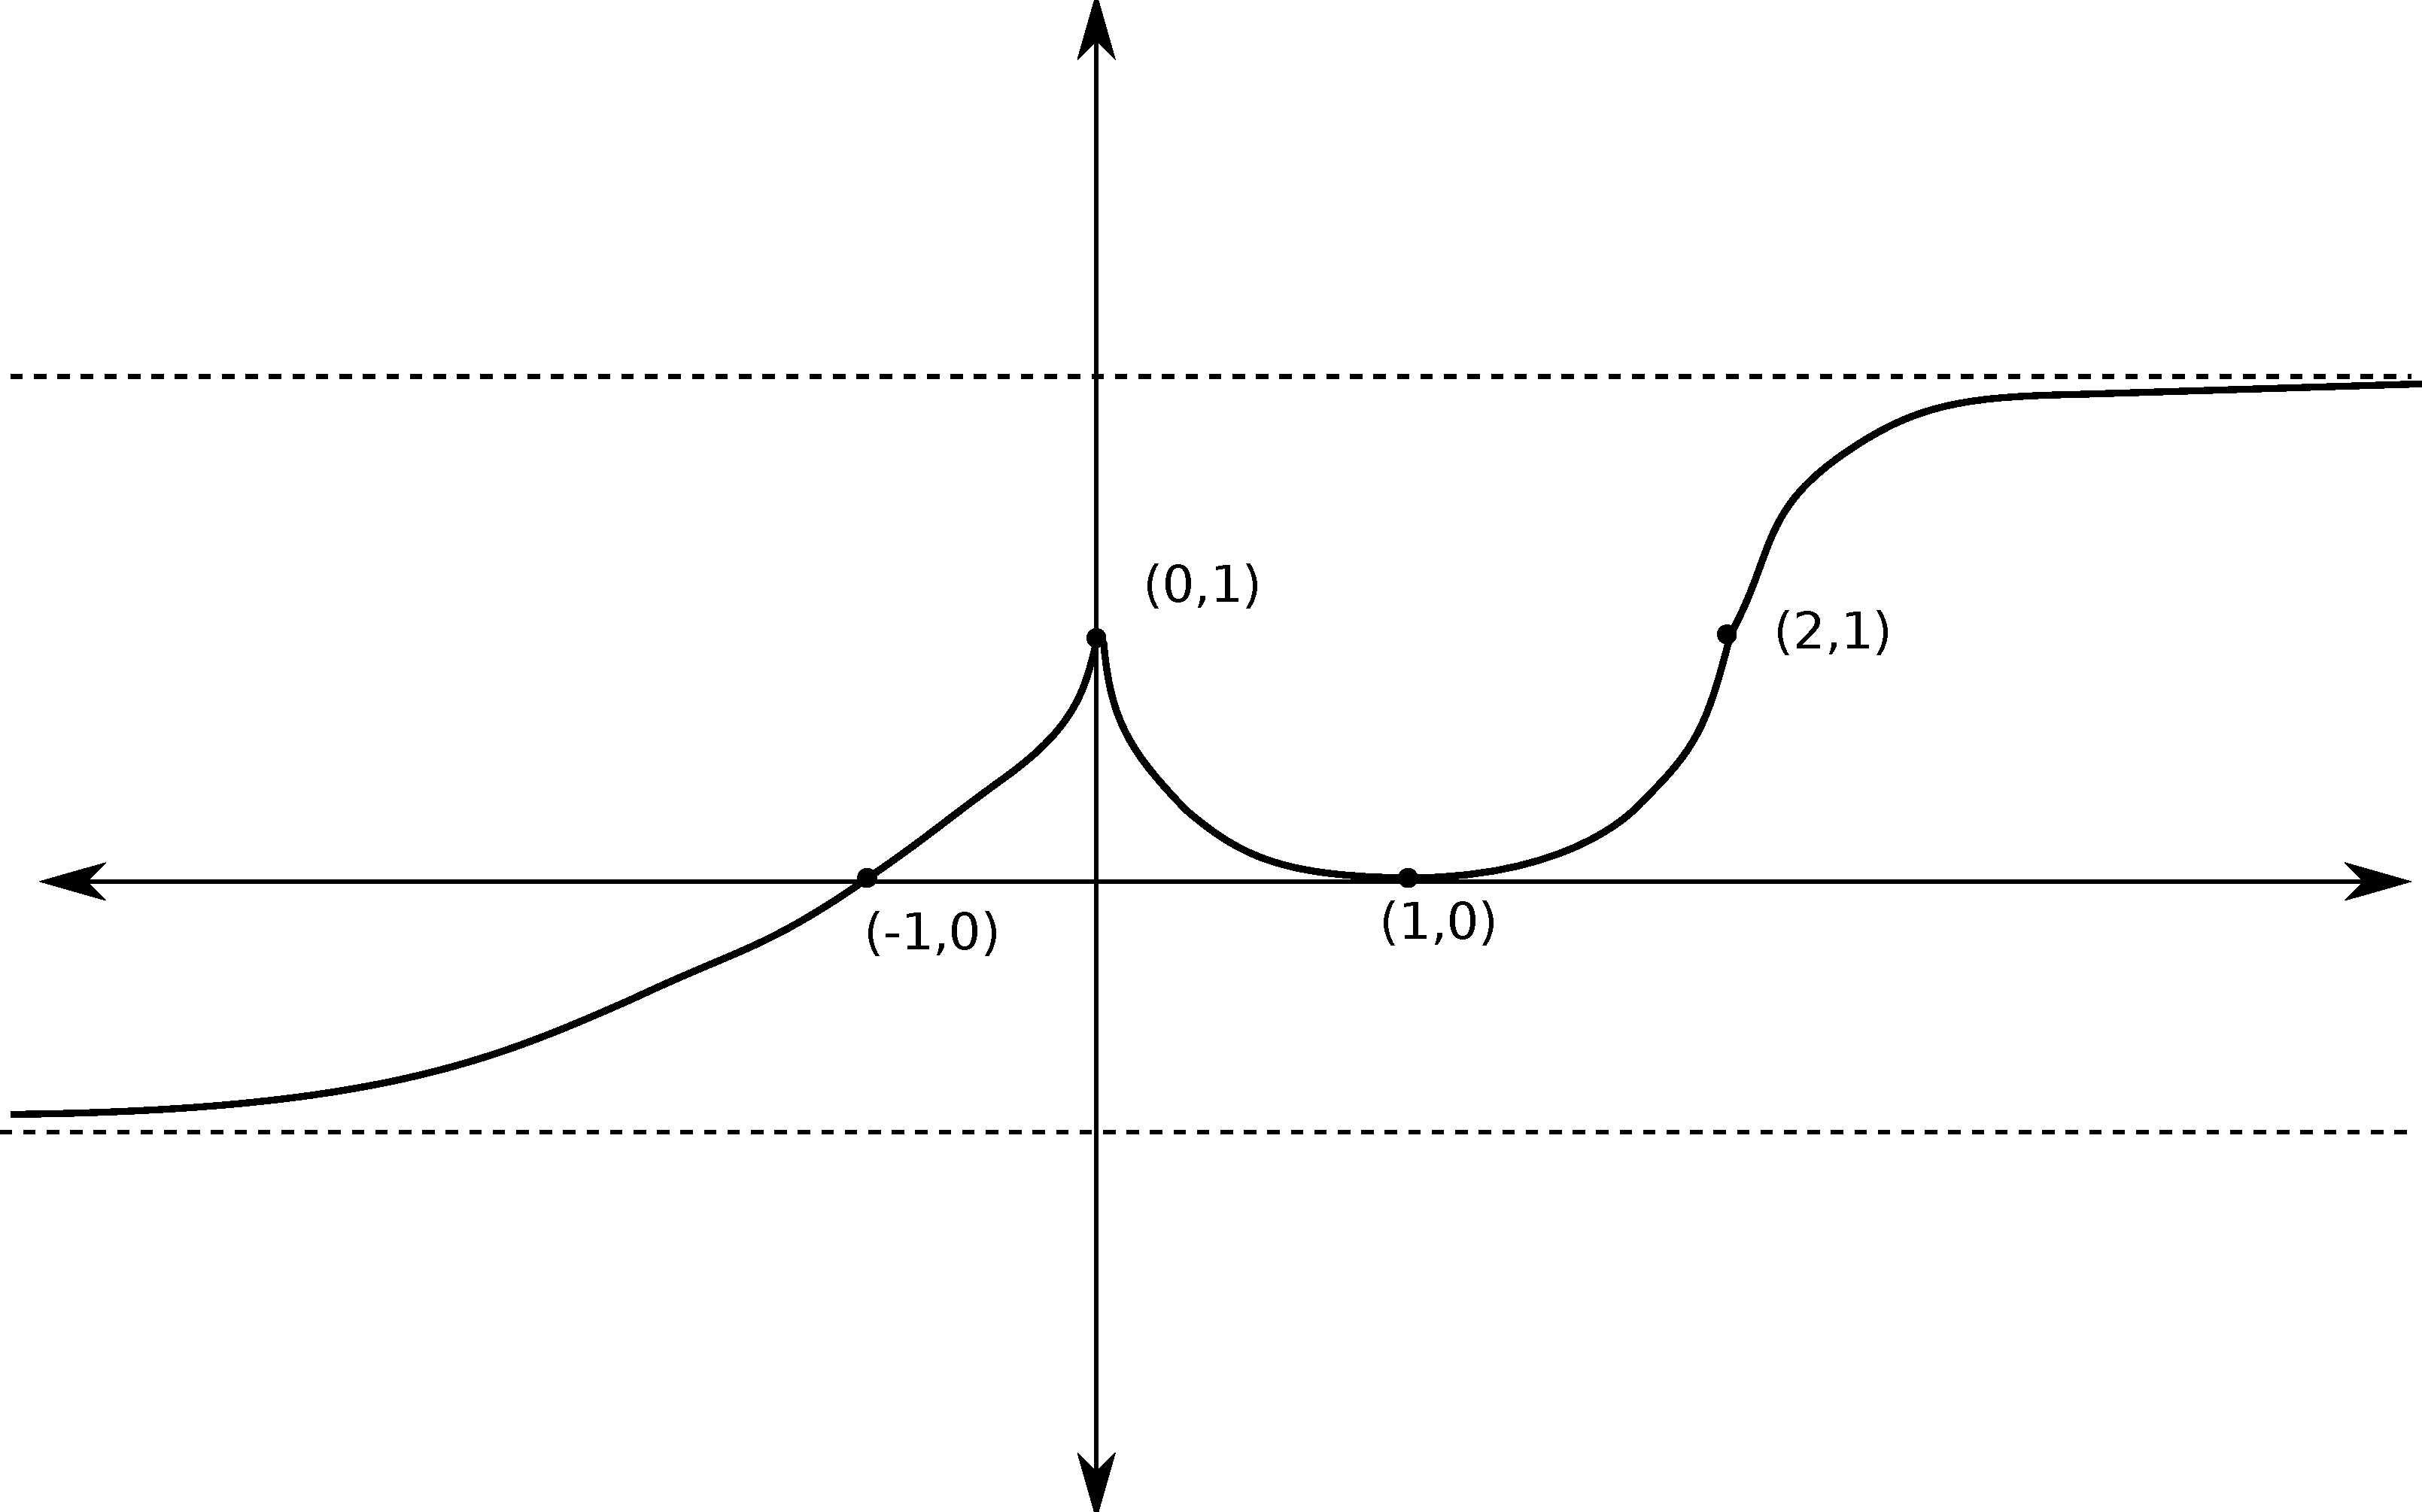
\includegraphics[width=0.8\textwidth]{A3_3}
\end{center}
 \end{enumerate}

\end{document}
 
